
%New colors defined below
\definecolor{codegreen}{rgb}{0,0.6,0}
\definecolor{codegray}{rgb}{0.5,0.5,0.5}
\definecolor{codepurple}{rgb}{0.58,0,0.82}
\definecolor{backcolour}{rgb}{0.95,0.95,0.92}

%Code listing style named "mystyle"
\lstdefinestyle{mystyle}{
  backgroundcolor=\color{backcolour},   commentstyle=\color{codegreen},
  keywordstyle=\color{magenta},
  numberstyle=\tiny\color{codegray},
  stringstyle=\color{codepurple},
  basicstyle=\ttfamily\footnotesize,
  breakatwhitespace=false,
  breaklines=true,
  captionpos=b,
  keepspaces=true,
  numbers=left,
  numbersep=5pt,
  showspaces=false,
  showstringspaces=false,
  showtabs=false,
  tabsize=2
}

%"mystyle" code listing set
\lstset{style=mystyle}

\chapter{Implementation} \label{implementation}

\section{Encoding algorithm}
The original NanoJPEG library, written in C, has an API composed of two main functions: \texttt{njDecode()}, which receives raw JPEG data in a byte array and does the actual decoding, and \texttt{njGetImage()}, which copies the decoded image from an internal buffer back to the caller. The whole library uses a static state structure, so it is not thread-safe, however passing the state structure as parameter would allow multithreading.

% \begin{lstlisting}
% bool writeJpeg(WRITE_ONE_BYTE output, const void* pixels_, unsigned short width, unsigned short height, bool isRGB, unsigned char quality_, bool downsample, const char* comment)
% \end{lstlisting}
% It accepts, in order:
% \begin{itemize}
%     \item the output writer buffer;
%     \item the pixels of the image;
%     \item width and height dimensions;
%     \item a flag to select if it is RGB or grayscale;
%     \item a value between 0 and 100 for the quality;
%     \item a downsample flag to select if use YCbCr 4:4:4 or 4:2:0;
%     \item a comment for the JFIF header. 
% \end{itemize}

Decompressing a JPEG image is simpler than creating it for three reasons: the input size is already known (the output size is fixed by width and height), there is no quality setting (the quantization table is already known), and there are no choices to be made about the compression (the Huffman table us already known).\\
Decompressing JPEG images could also be complicated by the myriad legal combinations of color spaces and representation formats and advanced features. NanoJPEG deals with this complexity by supporting only a core set of features, that in practice cover most use cases: only a few color spaces (YCbCr, RGB and single channel) are supported with any integer subsampling ratio on any channel, and no progressive scan (which is the most immediate limit of the library).

Although the order in which the specific functions are called is slightly different, the data flow can be summarized as:
\begin{itemize}
    \item Read 8x8 data blocks from stream
    \begin{itemize}
        \item Read DC differential coefficient and compute DC coefficient (sum of last DC coef and difference)
        \item Read Huffman Variable Length Codes until end of block (function \texttt{njGetVLC()})
        \item Convert from Huffman code to numeric value using the correct code for the component
        \item De-quantize or rescale AC coefficients: multiply each by the corresponding value in the correct Quantization Table for the component
    \end{itemize}
    \item Inverse Discrete Cosine Transform (IDCT) (functions \texttt{njRowIDCT()} and \texttt{njColIDCT()})
    \item rescaling of components which are downsampled (functions \texttt{njUpsampleH()} and \texttt{njUpsampleV()} called inside \texttt{njConvert()})
    \item Convert to RGB color space if different (inside function \texttt{njConvert()})
    \item Copy back to user buffer (separate user API call, function \texttt{njGetImage()})
\end{itemize}
Of these phases, the read and write phases cannot be processed on a GPGPU because they are inherently serial.\\
The other phases can exploit parallel computing since any pixel depends at most from a few neighboring pixels.

\section{NanoJPEG CUDA Implementation Details}

NanoJPEG CUDA compiles with the standard \texttt{nvcc} compiler.\\
The library allows the user of the API to disable all CUDA features, by setting to zero the parameter \texttt{use\_cuda} of function \texttt{njInit()}.

The block diagram of the CUDA version of the library is shown in \autoref{fig:nanojpeg_diag}.
\begin{figure}[h]
    \centering
    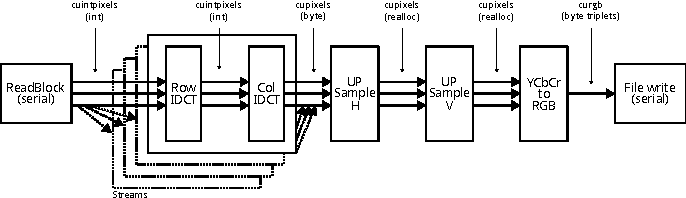
\includegraphics[width=1\textwidth]{Pictures/flow01.pdf}
    \caption{Data flow of NanoJPEG CUDA}
    \label{fig:nanojpeg_diag}
\end{figure}

NanoJPEG CUDA is divided into two main parts: function \texttt{\textbf{njCudaDecodeScan()}} handles from input data up to the IDCT, while function \texttt{\textbf{njCudaConvert()}} handles upsampling and RGB color space conversion.

Read from stream, Huffman decoding and de-quantization are implemented in function \texttt{njReadBlock()}, which is CPU-only.

The bi-dimensional IDCT is implemented as two separate functions, \texttt{njCudaRowIDCT()} and \texttt{njCudaRowIDCT()}.

The image is divided into four horizontal slices. When \texttt{njReadBlock()} finishes reading one slice, \texttt{njCudaRowIDCT()} and \texttt{njCudaRowIDCT()} are executed for that slice. The IDCTs for the four slices are executed in four separate CUDA streams so that an initial \texttt{CudaMemcpyAsync()} and the IDCT kernels can run on the GPU while the CPU reads the next slice from file. As a result, the starting times of the IDCTs in the four streams are staggered. This allows to reduce non-parallelizable task time at the beginning of the algorithm, since only a quarter of the file needs to be read before the GPU can start.

The program is disk-bound anyway, so a lower number of threads (as low as 2) could in theory be used, alternating the execution of the IDCT kernels between the first and the second, optionally subdividing the IDCT task in more than 4 slices. However the speed gain would be very small, most probably negated by the kernel setup time. Also, the creation of streams is comparatively cheap, so the solution using four streams was chosen.\\
\autoref{fig:streams} shows the sequence of kernel executions.

\begin{figure}
    \centering
    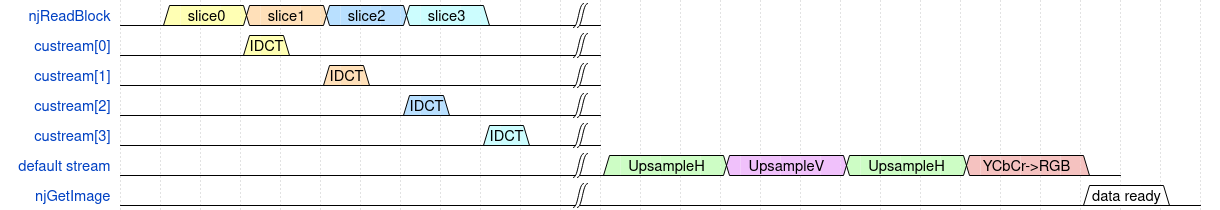
\includegraphics[width=1\textwidth]{Pictures/wavedrom_sequenza.png}
    \caption{Execution timeline}
    \label{fig:streams}
\end{figure}

Upsampling is optional, depending on the content of the file. In general functions \texttt{njCudaUpsampleH()} and \texttt{njCudaUpsampleV()} can be executed many times on any component, each doubles the size of the image in the horizontal or vertical axis respectively.

Eventually the image is converted back to the RGB format, which is a simple linear function implemented in integer arithmetic.

\section{Test application nanoex.cu}
The test application provided with the library (\texttt{nanoex.cu}) simply reads a JPEG file, decodes it using NanoJPEG, and writes the uncompressed result to a PPM file.

The test program received minor modifications to test NanoJPEG CUDA.

A new command-line option \texttt{"-nocuda"} was added to test the non-CUDA version of the library.